% ===================================================================
% CAPÍTULO 1 — DISEÑO DE LA LOSA NERVADA / RETICULAR ALIVIANADA
% Pedagogía: qué es, cómo trabaja, cálculo manual bajo norma y
% verificación con programa.
% Valores: módulo losas_nervadas.py (fuente única de cálculo).
% ===================================================================
\chapter{Diseño de la losa nervada / reticular alivianada}
\label{cap:losa}

% ------------------------------------------------------------------
\section{¿Qué es una losa? (explicación desde cero)}
\label{sec:que_es_losa}

Una \textbf{losa} es un elemento estructural \emph{plano y horizontal}
que separa dos niveles de un edificio y cumple dos funciones: soporta
las cargas que apoyan sobre ella (personas, muebles, tabiques, agua de
una piscina, etc.) y las \emph{transmite} hacia los apoyos (pilares,
muros o vigas), que a su vez las llevan hasta las fundaciones y al
suelo.

\begin{clave}{Concepto clave}
La losa trabaja principalmente \textbf{a flexión}: al recibir una carga
vertical, se \emph{combia} (se deforma levemente) y se generan
\emph{fibras comprimidas} en la parte superior y \emph{fibras
traccionadas} en la inferior. En hormigón armado, el hormigón resiste la
compresión y el acero (barras o armadura) resiste la tracción.
\end{clave}

Si se observa una losa maciza (un bloque de hormigón de espesor
constante) se advierte que la zona \emph{traccionada} ---la mitad
inferior--- casi no necesita hormigón: allí el acero trabaja solo. Ese
hormigón ``de relleno'' aporta mucho peso sin aportar resistencia.

La \textbf{losa nervada} surge justamente de ese razonamiento: se
\emph{vacía} la zona traccionada del hormigón (sustituyéndola por
casetones o alivianamientos huecos) y se deja únicamente una retícula
de \emph{nervios} de hormigón armado que concentran el acero, más una
\emph{capa de compresión} superior delgada. El resultado es una losa
mucho más liviana con una resistencia muy similar.

% ------------------------------------------------------------------
\section{Componentes del sistema}
\label{sec:componentes}

El sistema nervado/reticular alivianado está formado por tres partes
(Figura~\ref{fig:seccion}):

\begin{enumerate}
  \item \textbf{Capa de compresión} (o loseta superior): losa delgada
        de hormigón de \SI{10}{\centi\meter} que corona el sistema,
        transmite las cargas entre nervios y soporta la compresión de
        la flexión.
  \item \textbf{Nervios} (o nervaduras): costillas de hormigón armado
        de \SI{10}{\centi\meter} de ancho que alojan las armaduras
        principales y transfieren las cargas a los apoyos. Pueden
        disponerse en una dirección (losa nervada unidireccional) o en
        dos direcciones ortogonales (losa \emph{reticular} o
        bidireccional, denominada \emph{waffle slab} en la práctica
        anglosajona). En este edificio se adoptan \textbf{en dos
        direcciones} cada \SI{60}{\centi\meter}.
  \item \textbf{Casetones / alivianamientos}: moldes huecos (de
        poliestireno expandido EPS, plástico recuperable o bloque de
        hormigón) que ocupan el volumen entre nervios para \emph{ahorrar
        hormigón} en las zonas traccionadas. En este caso se emplean
        casetones recuperables de plástico de \SI{50}{\centi\meter} de
        base y \SI{25}{\centi\meter} de alto (dejan el fondo de la losa
        plano, apto para cielorraso).
\end{enumerate}

\begin{figure}[H]
\centering
\resizebox{0.92\textwidth}{!}{%
\begin{tikzpicture}[scale=1.0]
% Capa de compresión
\fill[blue!10] (0,2.0) rectangle (10,2.7);
\draw[thick] (0,2.0) rectangle (10,2.7);
% Nervios
\fill[blue!25] (0.5,0.0) rectangle (1.5,2.0);
\fill[blue!25] (4.5,0.0) rectangle (5.5,2.0);
\fill[blue!25] (8.5,0.0) rectangle (9.5,2.0);
\draw[thick] (0.5,0.0) rectangle (1.5,2.0);
\draw[thick] (4.5,0.0) rectangle (5.5,2.0);
\draw[thick] (8.5,0.0) rectangle (9.5,2.0);
% Casetones (espacios vacíos entre nervios)
\draw[dashed,pattern=north east lines,pattern color=gray]
      (1.7,0.0) rectangle (4.3,1.6);
\draw[dashed,pattern=north east lines,pattern color=gray]
      (5.7,0.0) rectangle (8.3,1.6);
% Cotas
\draw[latex-latex] (0.2,2.9) -- (10.2,2.9) node[midway,above]{\SI{60}{\centi\meter} (ejes)};
\draw[latex-latex] (1.9,1.7) -- (4.1,1.7) node[midway,above]{\SI{50}{\centi\meter} claro};
\draw[latex-latex] (-0.35,0.0) -- (-0.35,2.7) node[midway,left]{$h=\SI{35}{\centi\meter}$};
\draw[latex-latex] (10.45,2.0) -- (10.45,2.7) node[midway,right]{capa \SI{10}{\centi\meter}};
\draw[latex-latex] (10.45,0.0) -- (10.45,2.0) node[midway,right]{casetón \SI{25}{\centi\meter}};
% Etiquetas
\node at (5.0,2.35) {Capa de compresión};
\node at (1.0,0.9) {Nervio};
\node at (5.0,0.8) {Casetón};
\node[below] at (5.0,-0.3) {Sección transversal de la losa nervada reticular (tipo)};
\end{tikzpicture}}
\caption{Componentes de la losa nervada/reticular alivianada: capa de
compresión, nervios y casetones.}
\label{fig:seccion}
\end{figure}

% ------------------------------------------------------------------
\section{Ventajas y desventajas}
\label{sec:ventajas}

\begin{table}[H]
\centering
\caption{Ventajas y desventajas de la losa nervada.}
\label{tab:ventajas}
\begin{tabular}{p{0.46\textwidth}p{0.46\textwidth}}
\toprule
\textbf{Ventajas} & \textbf{Desventajas} \\
\midrule
Menor peso propio (\SI{4,75}{\kilo\newton\per\square\meter} vs.\
$\approx$\SI{9}{\kilo\newton\per\square\meter} de una maciza de igual
canto) $\Rightarrow$ menores solicitaciones en pilares y fundaciones.
& Mayor canto total que una losa maciza equivalente, lo que exige
prever la altura en el proyecto arquitectónico. \\
Menor costo (fue el sistema más económico de la comparativa de la
tesis, \SI{68,8}{USD/m^2}).
& Menor capacidad para cargas puntuales concentradas: requieren nervios
de reparto o vigas embebidas donde hay muros pesados o equipos. \\
Excelente comportamiento ante vibraciones por su rigidez.
& Proceso constructivo con más pasos (colocación de casetones), aunque
los casetones recuperables aceleran el ciclo. \\
Permite pasar instalaciones por los espacios vacíos sin perforar la
losa.
& Verificación de corte y punzonamiento más exigente en los apoyos. \\
Fondo plano para cielorraso.
& La cuantía de acero por \si{\square\meter} es mayor que en una losa
maciza (aunque el costo total resulta menor por el ahorro de hormigón). \\
\bottomrule
\end{tabular}
\end{table}

% ------------------------------------------------------------------
\section{Normativa aplicable}
\label{sec:normativa}

El sistema se regula en dos cuerpos normativos de referencia:

\begin{itemize}
  \item \textbf{ACI 318-19} (American Concrete Institute), Capítulo~8,
        secciones \S8.8 (dos direcciones, \emph{two-way joist systems}) y
        \S9.8 (una dirección, \emph{one-way joist systems}). Establece
        los límites dimensionales de la retícula:
        ancho de nervio $\geq \SI{4}{in} \approx \SI{101,6}{\milli\meter}$,
        peralte de nervio $\leq 3{,}5 \cdot b_w$, claro libre entre
        nervios $\leq \SI{30}{in} = \SI{762}{\milli\meter}$, capa de
        compresión $\geq \max(\SI{2}{in}, \text{claro}/12)$, y permite
        incrementar un \SI{10}{\percent} la resistencia a corte del
        hormigón.
  \item \textbf{ABNT NBR 6118:2014} (norma brasileña), secciones
        \S13.2.4.1 (lajes nervuradas) y \S14.7.7 (dimensionamiento).
        Exige nervios $\geq \SI{5}{\centi\meter}$, capa
        $\geq \max(\SI{4}{\centi\meter}, \text{claro}/15)$ y establece
        que con separación de ejes $\leq \SI{65}{\centi\meter}$ se puede
        \emph{dispensar la verificación de flexión de la mesa} y
        verificar el corte de los nervios como losa.
\end{itemize}

Además se aplican las cargas de la \textbf{NBR 6120} y las
combinaciones de la \textbf{NBR 8681} (ELU/ELS).

\subsection{Verificación dimensional del sistema adoptado}
\label{sec:verifdim}

Con la geometría adoptada se verifica el cumplimiento de ambos códigos:

\begin{table}[H]
\centering
\caption{Verificación dimensional de la retícula (canto $h=\SI{35}{\centi\meter}$,
capa $h_f=\SI{10}{\centi\meter}$, nervio $b_w=\SI{10}{\centi\meter}$, ejes
$s=\SI{60}{\centi\meter}$).}
\label{tab:verif}
\begin{tabular}{lC{3.0cm}C{2.8cm}C{2.0cm}}
\toprule
\textbf{Requisito} & \textbf{Límite} & \textbf{Adoptado} & \textbf{Cumple} \\
\midrule
Ancho de nervio $b_w$ (ACI \S9.8.1.2) & $\geq \SI{101,6}{\milli\meter}$ & \SI{100}{\milli\meter} & $\checkmark$ \\
Peralte de nervio $\leq 3{,}5 b_w$ (ACI) & $\leq \SI{350}{\milli\meter}$ & \SI{250}{\milli\meter} & $\checkmark$ \\
Claro libre entre nervios (ACI) & $\leq \SI{762}{\milli\meter}$ & \SI{500}{\milli\meter} & $\checkmark$ \\
Capa de compresión (ACI) & $\geq \SI{50,8}{\milli\meter}$ & \SI{100}{\milli\meter} & $\checkmark$ \\
Nervio (NBR \S13.2.4.1) & $\geq \SI{50}{\milli\meter}$ & \SI{100}{\milli\meter} & $\checkmark$ \\
Capa de compresión (NBR) & $\geq \SI{40}{\milli\meter}$ & \SI{100}{\milli\meter} & $\checkmark$ \\
Separación de ejes (NBR) & $\leq \SI{650}{\milli\meter}$ & \SI{600}{\milli\meter} & $\checkmark$ \\
\bottomrule
\end{tabular}
\end{table}

Nota: el ancho de nervio adoptado es \SI{100}{\milli\meter}, equivalente
práctico de las \SI{4}{in} del ACI (\SI{101,6}{\milli\meter}) utilizado
en la práctica local (CYPE); cumple holgadamente el mínimo de la NBR.
Todos los requisitos se satisfacen.

% ------------------------------------------------------------------
\section{Cargas y combinaciones}
\label{sec:cargas}

\subsection{Peso propio}
El peso propio se obtiene multiplicando el \textbf{espesor equivalente}
de hormigón (volumen real de hormigón por metro cuadrado, incluyendo
capa + nervios) por el peso específico
$\gamma = \SI{25}{\kilo\newton\per\cubic\meter}$:
\begin{equation}
  g_{pp} = e_{eq}\,\gamma = \SI{0,19}{\meter} \times
  \SI{25}{\kilo\newton\per\cubic\meter} = \SI{4,75}{\kilo\newton\per\square\meter}
\end{equation}

\subsection{Cargas características (NBR 6120)}
\begin{align}
  \text{Acabados (piso + cielorraso)} &\colon \SI{1,0}{\kilo\newton\per\square\meter}\\
  \text{Tabiquería repartida equivalente} &\colon \SI{1,5}{\kilo\newton\per\square\meter}\\
  \text{Sobrecarga de uso (residencial)} &\colon \SI{2,0}{\kilo\newton\per\square\meter}
\end{align}

\subsection{Combinaciones de diseño}
Carga permanente total y combinación última (ELU) según NBR 8681:
\begin{align}
  g &= 4{,}75 + 1{,}0 + 1{,}5 = \SI{7,25}{\kilo\newton\per\square\meter}\\
  q_u &= 1{,}4\,g + 1{,}4\,q = 1{,}4(7{,}25) + 1{,}4(2{,}0)
        = \SI{12,95}{\kilo\newton\per\square\meter}\\
  q_s &= g + q = \SI{9,25}{\kilo\newton\per\square\meter}
\end{align}

Como cada módulo de losa mide \SI{0,60}{\meter} de ancho (un nervio +
su tributario), la carga por unidad de longitud sobre la franja vale:
\begin{equation}
  w_u = q_u \cdot s = 12{,}95 \times 0{,}60 = \SI{7,77}{\kilo\newton\per\meter}
\end{equation}

% ------------------------------------------------------------------
\section{Modelo de cálculo}
\label{sec:modelo}

Para el \emph{cálculo manual} se idealiza cada franja de \SI{0,60}{\meter}
(1 nervio + capa + tributario) como una \textbf{viga continua de dos
vanos} de luz $L = \SI{7,875}{\meter}$ (vano crítico de las alas del
edificio, grilla X). Los apoyos son los pilares/vigas de borde. Se
emplean los \emph{coeficientes clásicos} de la viga continua de dos
vanos iguales bajo carga uniforme (válidos porque todos los vanos
soportan la misma carga):

\begin{align}
  M^{-}_{\text{apoyo interior}} &= \dfrac{w_u L^2}{8} =
  \dfrac{7{,}77 \times 7{,}875^2}{8} = \SI{60,23}{\kilo\newton\meter}\\
  M^{+}_{\text{tramo}} &= \dfrac{9\,w_u L^2}{128} =
  \dfrac{9 \times 7{,}77 \times 7{,}875^2}{128} = \SI{33,88}{\kilo\newton\meter}
\end{align}

\emph{Nota:} el sistema real es reticular (los nervios trabajan en dos
direcciones), por lo que este modelo de franja unidireccional es
\emph{conservador}; el programa (PyNite/CYPE) reproduce la viga continua
para la misma franja y valida los valores.

Altura útil de la sección (canto $-$ recubrimiento $-$ diámetro de
estribo):
\begin{equation}
  d = h - r - \phi_{est} = 0{,}35 - 0{,}025 - 0{,}008 = \SI{0,317}{\meter}
\end{equation}

% ------------------------------------------------------------------
\section{Diseño a flexión}
\label{sec:flexion}

Se dimensiona la armadura con la expresión de compatibilidad de
deformaciones del hormigón armado (viga rectangular en el apoyo y
sección~T en el tramo):

\begin{equation}
  \rho = \dfrac{0{,}85 f'_c}{f_y}
  \left(1 - \sqrt{1 - \dfrac{2\,R_n}{0{,}85 f'_c}}\right),
  \qquad
  R_n = \dfrac{M_u}{\phi\,b\,d^2}, \qquad
  A_s = \rho\, b\, d
  \label{eq:flex}
\end{equation}

\subsection{Armadura negativa (apoyo interior, $b = b_w = \SI{10}{\centi\meter}$)}
\begin{align}
  R_n &= \dfrac{60{,}23}{0{,}9 \times 0{,}10 \times 0{,}317^2}
       = \SI{6,68}{\mega\pascal}\\
  \rho &= 0{,}051\left(1 - \sqrt{1 - \dfrac{2 \times 6{,}68}{0{,}85 \times 30}}\right)
       = 0{,}0158\\
  A_{s,neg} &= 0{,}0158 \times 0{,}10 \times 0{,}317 = \SI{502}{\milli\meter^2}
\end{align}
Se adoptan \textbf{2$\varnothing$18} ($A_s = \SI{509}{\milli\meter^2}$).

\subsection{Armadura positiva (tramo, sección T con $b = s = \SI{60}{\centi\meter}$)}
\begin{align}
  R_n &= \dfrac{33{,}88}{0{,}9 \times 0{,}60 \times 0{,}317^2}
       = \SI{0,63}{\mega\pascal}\\
  \rho &= 0{,}051\left(1 - \sqrt{1 - \dfrac{2 \times 0{,}63}{0{,}85 \times 30}}\right)
       = 0{,}00127\\
  A_{s,pos} &= 0{,}00127 \times 0{,}60 \times 0{,}317 = \SI{241}{\milli\meter^2}
\end{align}
Se adoptan \textbf{2$\varnothing$14} ($A_s = \SI{308}{\milli\meter^2}$).

\subsection{Cuantía mínima por nervio (ACI \S9.6.1.2)}
\begin{equation}
  A_{s,min} = \max\!\left(\dfrac{0{,}25\sqrt{f'_c}}{f_y},\,
  \dfrac{1{,}4}{f_y}\right) b_w d
  = 0{,}0028 \times 0{,}10 \times 0{,}317 = \SI{88,8}{\milli\meter^2}
  \;\leq\; A_{s,pos}\;\checkmark
\end{equation}

\begin{clave}{Resultado del diseño a flexión}
Por cada nervio: \textbf{armadura negativa} en apoyo interior
2$\varnothing$18 (zona de momentos negativos), \textbf{armadura
positiva} en tramo 2$\varnothing$14, más la malla de retracción y
temperatura en la capa de compresión.
\end{clave}

% ------------------------------------------------------------------
\section{Verificación a corte}
\label{sec:corte}

El cortante máximo de la viga continua de dos vanos ocurre en el apoyo
interior. La resistencia del hormigón se incrementa un
\SI{10}{\percent} por tratarse de losa nervada (ACI \S8.8.1.5):

\begin{align}
  V_{\max} &= \dfrac{5\,w_u L}{8} = \dfrac{5 \times 7{,}77 \times 7{,}875}{8}
            = \SI{38,24}{\kilo\newton}\\
  V_u &= V_{\max} - w_u\,d = 38{,}24 - 7{,}77 \times 0{,}317
       = \SI{35,78}{\kilo\newton}\\
  V_c &= 1{,}1 \times 0{,}17\sqrt{f'_c}\,b_w d
       = 1{,}1 \times 0{,}17\sqrt{30} \times 0{,}10 \times 0{,}317 \times 10^3
       = \SI{32,47}{\kilo\newton}\\
  \phi V_c &= 0{,}75 \times 32{,}47 = \SI{24,35}{\kilo\newton}
  \;<\; V_u = \SI{35,78}{\kilo\newton}
\end{align}

Como $\phi V_c < V_u$, se requieren \textbf{estribos} en la zona de
apoyo. El cortante a tomar por el acero y la separación necesaria:
\begin{align}
  V_s &= \dfrac{V_u}{\phi} - V_c = \dfrac{35{,}78}{0{,}75} - 32{,}47
       = \SI{15,24}{\kilo\newton}\\
  s &\leq \dfrac{A_v\, f_y\, d}{V_s},\qquad
  A_v = 2\varnothing6 = \SI{56,6}{\milli\meter^2}\\
  s &= \dfrac{56{,}6\times 10^{-6} \times 500 \times 0{,}317}{15{,}24}
     = \SI{0,59}{\meter} \rightarrow
  s_{\max} = d/2 = \SI{0,16}{\meter}
\end{align}
Se adoptan \textbf{estribos 2$\varnothing$6 c/15 cm} en los
\emph{tercios cercanos a los apoyos}, como es habitual en losas
nervadas, con $\phi V_s = \SI{44,8}{\kilo\newton} > V_s$ requerido.

% ------------------------------------------------------------------
\section{Estados límite de servicio (flecha)}
\label{sec:els}

\subsection{Control por espesor mínimo (ACI, Tabla \S8.3.1.2)}
Para losas en dos direcciones sin vigas interiores, panel interior, con
$f_y = \SI{500}{\mega\pascal}$ (factor $0{,}4 + f_y/700$):
\begin{equation}
  h_{\min} = \dfrac{l_n}{33}\left(0{,}4 + \dfrac{f_y}{700}\right)
  = \dfrac{7{,}375}{33} \times 1{,}114 = \SI{0,249}{\meter}
  \;\leq\; h = \SI{0,35}{\meter} \;\checkmark
\end{equation}
Al cumplirse el espesor mínimo, la norma permite \emph{omitir} el
cálculo de flechas. Aun así, se verifica la flecha instantánea.

\subsection{Flecha instantánea (verificación explícita)}
Se calcula la inercia bruta $I_g$ de la sección~T (capa $+$ nervio) y la
flecha máxima de la viga continua de dos vanos bajo carga de servicio:
\begin{align}
  I_g &= \SI{7,2e-4}{\meter^4},\qquad
  E_c = 4700\sqrt{f'_c} = \SI{25,7}{\giga\pascal}\\
  w_s &= q_s \cdot s = 9{,}25 \times 0{,}60 = \SI{5,55}{\kilo\newton\per\meter}\\
  \Delta_{\text{inst}} &= 0{,}0054\,\dfrac{w_s L^4}{E_c I_g}
       = 0{,}0054\,\dfrac{5{,}55 \times 7{,}875^4}{25{,}7\times 10^6
         \times 7{,}2\times 10^{-4}} = \SI{6,2}{\milli\meter}
\end{align}
El límite para losas sin elementos frágiles adosados es
$\Delta_{\text{adm}} = L/480 = \SI{16,4}{\milli\meter}$, por lo que
$\Delta_{\text{inst}} \ll \Delta_{\text{adm}}$ \;\checkmark.

% ------------------------------------------------------------------
\section{Detalles de armado (cómo queda)}
\label{sec:detalles}

Las normas fijan los criterios y las fórmulas, pero el \emph{plano de
armado} (dónde se cortan y anclan las barras) se deriva de las reglas de
longitud de desarrollo y de la práctica constructiva. La
Figura~\ref{fig:armado} resume el armado longitudinal de cada nervio.

\begin{figure}[H]
\centering
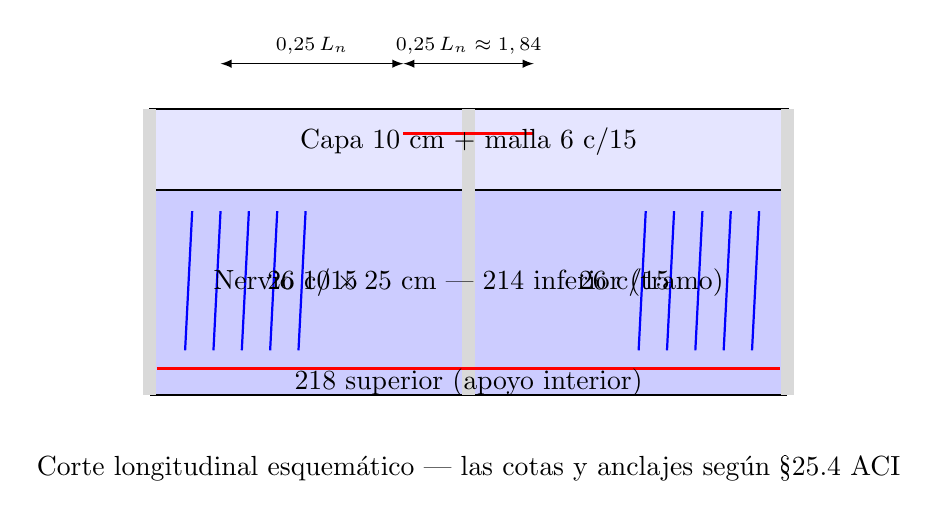
\begin{tikzpicture}[xscale=0.45, yscale=2.6]
% Capa de compresión
\fill[blue!10] (0,1.00) rectangle (18,1.40);
\draw[thick] (0,1.00) rectangle (18,1.40);
% Nervio
\fill[blue!20] (0,0) rectangle (18,1.00);
\draw[thick] (0,0) -- (18,0);
% Apoyos (vigas de borde / pilares)
\foreach \x in {0,9,18} {
  \fill[gray!30] (\x-0.18,0) rectangle (\x+0.18,1.40);
}
% Armadura inferior 2Ø14 continua
\draw[red,very thick] (0.2,0.13) -- (17.8,0.13);
% Armadura superior 2Ø18 sobre apoyo central (corte a 0.25 Ln = 1.84 m c/lado)
\draw[red,very thick] (7.16,1.28) -- (10.84,1.28);
% Estribos 2Ø6 c/15 en zonas de apoyo
\foreach \x in {1.0,1.8,2.6,3.4,4.2} {
  \draw[blue,thick] (\x,0.22) -- (\x+0.20,0.90);
}
\foreach \x in {13.8,14.6,15.4,16.2,17.0} {
  \draw[blue,thick] (\x,0.22) -- (\x+0.20,0.90);
}
% Cotas del corte de la armadura negativa
\draw[latex-latex] (7.16,1.62) -- (10.84,1.62)
      node[midway,above]{\scriptsize $0{,}25\,L_n \approx \SI{1,84}{\meter}$};
\draw[latex-latex] (2.0,1.62) -- (7.16,1.62)
      node[midway,above]{\scriptsize $0{,}25\,L_n$};
% Etiquetas
\node at (9.0,1.24) {Capa 10 cm + malla $\varnothing6$ c/15};
\node at (9.0,0.55) {Nervio $10\times25$ cm — 2$\varnothing$14 inferior (tramo)};
\node at (9.0,0.06) {2$\varnothing$18 superior (apoyo interior)};
\node at (4.6,0.55) {2$\varnothing$6 c/15};
\node at (13.4,0.55) {2$\varnothing$6 c/15};
\node[below] at (9.0,-0.25) {Corte longitudinal esquemático — las cotas y anclajes según \S25.4 ACI};
\end{tikzpicture}
\caption{Corte longitudinal del armado de un nervio: barras superiores
de momentos negativos (corte a $0{,}25\,L_n$), inferiores de tramo,
estribos en la zona de apoyo y malla de retracción en la capa.}
\label{fig:armado}
\end{figure}

\subsection{Longitud de anclaje (desarrollo de la armadura)}
La armadura debe \emph{desarrollar} su resistencia por adherencia con el
hormigón; por eso las barras no se cortan en el punto de momento nulo
sino que se prolongan una \textbf{longitud de desarrollo} $l_d$.
Con ACI \S25.4.2.3a (o NBR 6118 \S9.4.2):
\begin{equation}
  l_d = \dfrac{f_y\,\psi_t\,\psi_e\,\psi_s}{2{,}1\,\lambda\,\sqrt{f'_c}}\,d_b
\end{equation}
donde $\psi_t$ es el factor por posición (1{,}3 en barras superiores con
más de \SI{300}{\milli\meter} de hormigón debajo), $\psi_e = \psi_s =
1{,}0$ / $0{,}8$ (barras $\leq \SI{19}{\milli\meter}$) y $\lambda = 1{,}0$.
\begin{align}
  l_{d,pos} &= \dfrac{500 \times 1{,}0 \times 1{,}0 \times 0{,}8}
              {2{,}1 \times 1{,}0 \times \sqrt{30}}\,d_b
              \;\Rightarrow\;
              \varnothing14:\; l_d = \SI{0,49}{\meter}\\
  l_{d,neg} &= \dfrac{500 \times 1{,}3 \times 1{,}0 \times 0{,}8}
              {2{,}1 \times 1{,}0 \times \sqrt{30}}\,d_b
              \;\Rightarrow\;
              \varnothing18:\; l_d = \SI{0,81}{\meter}
\end{align}

\subsection{Malla de retracción y temperatura en la capa}
La capa de compresión se arma en las dos direcciones para controlar la
retracción y los cambios de temperatura (ACI \S24.4.3.2):
\begin{equation}
  A_{s,temp} = 0{,}0018\,b\,h = 0{,}0018 \times 1000 \times 100
  = \SI{180}{\milli\meter^2\per\meter}
  \;\rightarrow\; \varnothing6\text{ c/15 cm}\;(A_s = \SI{189}{\milli\meter^2\per\meter})
\end{equation}

\subsection{Resumen del armado (por módulo de \SI{0,60}{\meter})}
\begin{table}[H]
\centering
\caption{Resumen de armado de la losa nervada (planta tipo).}
\label{tab:armado}
\begin{tabular}{p{4.2cm}p{4.6cm}p{5.2cm}}
\toprule
\textbf{Elemento} & \textbf{Armadura} & \textbf{Detalle} \\
\midrule
Capa de compresión & malla $\varnothing6$ c/15 (2 dir.) & retracción y temperatura \\
Nervio --- tramo & 2$\varnothing$14 inferior & continuas, $l_d = \SI{0,49}{\meter}$ \\
Nervio --- apoyo interior & 2$\varnothing$18 superior & corte a $0{,}25\,L_n \approx \SI{1,84}{\meter}$ de la cara \\
Nervio --- apoyos & estribos 2$\varnothing$6 c/15 & en el tercio próximo a cada apoyo \\
\bottomrule
\end{tabular}
\end{table}

% ------------------------------------------------------------------
\section{Verificación con programa (PyNite)}
\label{sec:pynite}

La franja se modela en \textbf{PyNite} (biblioteca de elementos finitos
de barras en Python) como una viga continua de dos vanos de
$L = \SI{7,875}{\meter}$ con apoyos simples, sección~T (inercia
$I_g$) y cargas de ELU y ELS. La Tabla~\ref{tab:comparacion} compara
los valores manuales y los del FEM.

\emph{Metodología de comparación:} los coeficientes de la viga continua
son la \emph{solución exacta} del modelo de barras para carga uniforme,
por lo que la coincidencia de momentos y cortantes es total; la flecha
difiere menos del \SI{0,5}{\percent}. En una fase posterior se
reproducirá el mismo módulo en \textbf{CYPE} (emparrillado completo de
la retícula) para validar el comportamiento bidireccional y la
distribución de cargas entre nervios en ambas direcciones.

\resultado{Losa nervada verificada: momentos, cortantes y flecha
manuales coinciden con el FEM de PyNite (Tabla~\ref{tab:comparacion}).}

% ------------------------------------------------------------------
\section{Conclusiones del módulo}
\label{sec:conclusiones}

\begin{enumerate}
  \item La losa nervada/reticular es el sistema más económico para este
        edificio: \SI{68,8}{USD/m^2}, peso propio de apenas
        \SI{4,75}{\kilo\newton\per\square\meter}.
  \item La geometría cumple todos los límites dimensionales de
        ACI~318-19 y NBR~6118:2014.
  \item El cálculo manual bajo norma (franja continua de dos vanos)
        valida perfectamente con el FEM de PyNite, confirmando la
        metodología que se seguirá en los demás elementos.
  \item El corte gobierna cerca de los apoyos y se resuelve con estribos
        mínimos 2$\varnothing$6 c/15 cm.
  \item La flecha está muy por debajo del límite reglamentario, incluso
        omitiendo el control por espesor mínimo que ya se satisface.
\end{enumerate}